\documentclass[aspectratio=169]{beamer} % 16:9 aspect ratio for modern screens

% Theme settings
\usetheme{metropolis} % Minimalist theme
\usefonttheme{professionalfonts} % Font theme

% Packages
\usepackage[utf8]{inputenc} % Encoding
\usepackage[T1]{fontenc}   % Font encoding
\usepackage[ngerman]{babel} % German language
\usepackage{graphicx}       % For including images
\usepackage{amsmath, amssymb} % For math symbols
\usepackage{tikz}          % For creating diagrams
\usepackage{booktabs}      % For better tables
\usepackage[sfdefault]{FiraSans} % For FiraSans font
\usepackage{caption} % For customizing captions
\usepackage[backend=biber, style=authoryear]{biblatex} % For bibliography
\usepackage{csquotes} % For context-sensitive quotation marks

% Bibliography file
\addbibresource{Hadronen im Quarkmodell.bib}

% Title page settings
\title{Hadronen im Quarkmodell}
\subtitle{Eine physikalische Betrachtung}
\author{Dein Name}
\date{Datum}

\begin{document}
    
    % Title Slide
    \begin{frame}
        \titlepage
    \end{frame}
    
    % Table of Contents
    \begin{frame}{Inhaltsverzeichnis}
        \tableofcontents
    \end{frame}
    
    % Section: Einführung
    \section{Einführung}
    \begin{frame}{Einführung}
        \begin{block}{Ziel der Präsentation}
            \begin{itemize}
                \item Vorstellung der Grundlagen des Quarkmodells~\cite{C.Amsler.2017}
                \item Beschreibung der Hadronenstruktur~\cite{GellMann.1964}
                \item Diskussion aktueller Herausforderungen~\cite{Zweig.1964}~und~\cite{Zweig.1964b}
            \end{itemize}
        \end{block}
        \begin{figure}
            \centering
            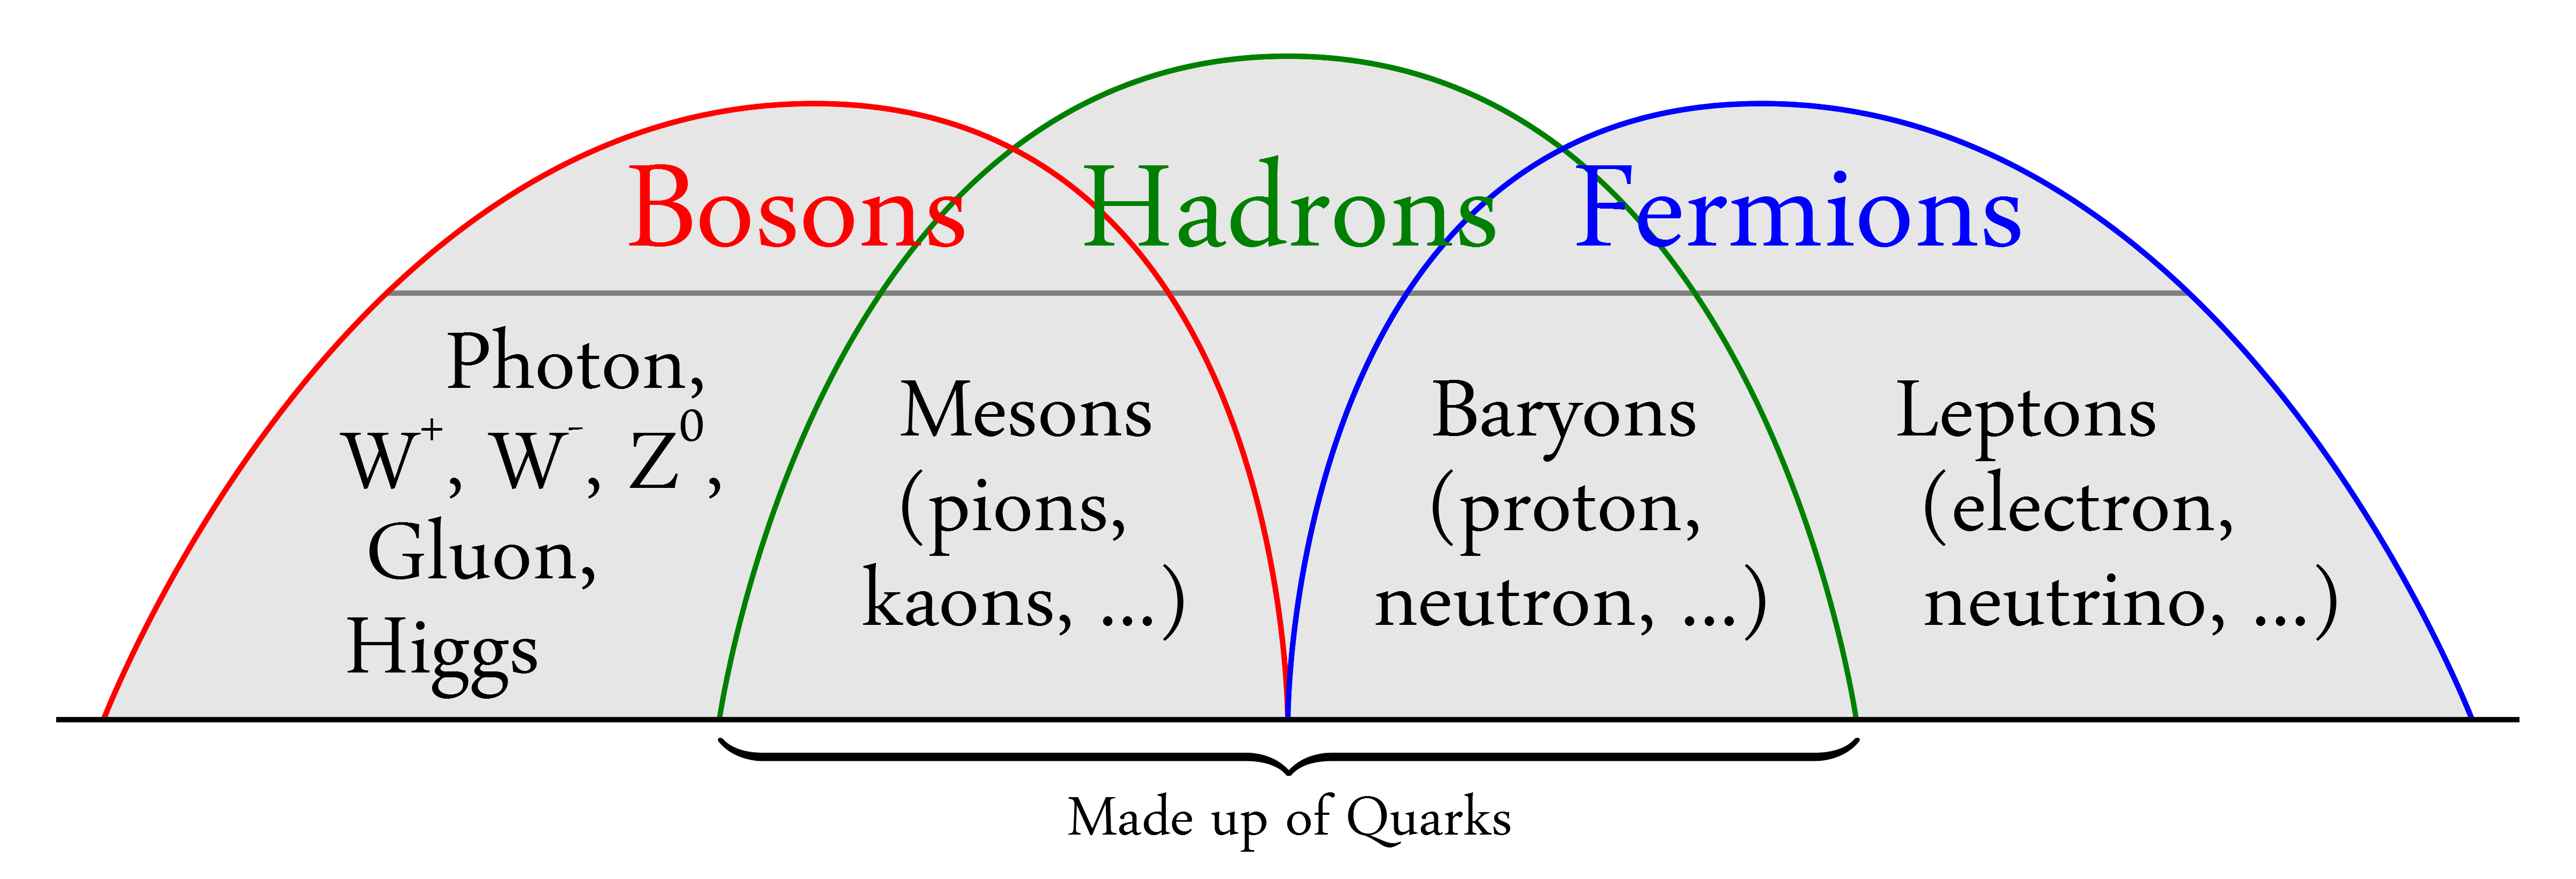
\includegraphics[width=0.6\linewidth]{Bosons-Hadrons-Fermions-RGB-png2.png}\footnote{aus \cite{Wikipedia.Standardmodell}: By Hugo Spinelli\nobreakspace-- Own work, CC0}
        \end{figure}
    \end{frame}
    
    % Section: Theoretische Grundlagen
    \section{Theoretische Grundlagen}
    \begin{frame}{Quarkmodell: Ein Überblick}
        \begin{itemize}
            \item Quarks als fundamentale Bausteine~\cite{Aaij.2015}
            \item Drei Farbladungen: Rot, Grün, Blau\cite{Wikipedia.Hadron}
            \item Austausch von Gluonen $\Rightarrow$ starke Wechselwirkung\cite{Aaij.2019}
        \end{itemize}
        \begin{equation}
            F = \frac{Gm_1m_2}{r^2} % Beispiel für eine Formel
        \end{equation}
    \end{frame}
    
    \begin{frame}{Hadronenklassen}
        \begin{block}{Baryonen}
            \begin{itemize}
                \item Drei Quarks
                \item Beispiele: Proton, Neutron
            \end{itemize}
        \end{block}
        \begin{block}{Mesonen}
            \begin{itemize}
                \item Ein Quark und ein Antiquark
                \item Beispiele: Pionen, Kaonen
            \end{itemize}
        \end{block}
    \end{frame}
    
    % Section: Experimentelle Beobachtungen
    \section{Experimentelle Beobachtungen}
    \begin{frame}{Nachweis von Quarks}
        \begin{figure}
            \centering
            \includegraphics[width=0.7\linewidth]{example-image} % Replace with actual image path
            \caption{Streuexperiment zur Quarkstruktur}
        \end{figure}
        \begin{itemize}
            \item Streuexperimente als zentrale Methode
            \item Nachweis von Quark-Ladungen
        \end{itemize}
    \end{frame}
    
    % Section: Zusammenfassung
    \section{Zusammenfassung}
    \begin{frame}{Schlussfolgerungen}
        \begin{itemize}
            \item Hadronen sind komplexe Strukturen aus Quarks
            \item Fortschritte in der Theorie und Experimente erforderlich
            \item Bedeutung des Quarkmodells für die moderne Physik
        \end{itemize}
    \end{frame}
    
    % Thank You Slide
    \begin{frame}{Vielen Dank!}
        \begin{center}
            \Huge Fragen?
        \end{center}
    \end{frame}
    
    % Bibliography
    \begin{frame}[allowframebreaks]{Literatur}
        \printbibliography
    \end{frame}
    
\end{document}